\documentclass[11pt]{scrartcl}

\usepackage[utf8]{inputenc} % Input encoding
\usepackage[T1]{fontenc} % Font encoding
\usepackage{siunitx} % Provides the \SI{}{} and \si{} command for typesetting SI units
\usepackage{graphicx} % Required for the inclusion of images
\usepackage{natbib} % Required to change bibliography style to APA
\usepackage{amsmath} % Required for some math elements 
\usepackage{lmodern} % Font used in the document
\usepackage{hyperref} % To add link in the document
\usepackage[headsepline]{scrpage2} % For headers and footers with KOMA classes
\usepackage{todonotes}
\usepackage{tikz, pgfplots}
\usepackage{pgfplotstable}
\usepackage{booktabs}
\usepackage{array}
\usepackage{colortbl}
\usepackage{enumitem} % Enumeration package
\usepackage[english]{babel} 

\synctex=1 % For syncing skim with Emacs

\setlength\parindent{0pt} % Removes all indentation from paragraphs

\renewcommand{\labelitemi}{\textbullet} % make items in itemize environment bullets rather that dashes
\renewcommand{\labelenumi}{\alph{enumi}.} % Make numbering in the enumerate environment by letter rather than
                                % number (e.g. section 6)

%\usepackage{times} % Uncomment to use the Times New Roman font

\usepackage{listings}
\usepackage[framed,autolinebreaks,useliterate]{mcode}

% Pgf cycle colors
\pgfplotsset{cycle list name = exotic, compat=1.12}


%----------------------------------------------------------------------------------------
%	DOCUMENT INFORMATION
%----------------------------------------------------------------------------------------

\addtokomafont{disposition}{\normalfont\bfseries} % Make title/sections/subsections font the same as the rest
                                % of the document

\title{Philip Morris: Data Analysis Improvement of Ciliary Beating of 3D Epithelial Tissue\\\vspace{1cm}Final report\vspace{1cm}} % Title

\author{Simon Jenni \& Laurent Hayez} % Author name

\date{\today} % Date for the report

\begin{document}

%----------------------------------------------------------------------------------------
%	HEADERS AND FOOTERS
%----------------------------------------------------------------------------------------

\setfootsepline[text]{.4pt}

\pagestyle{scrheadings}
\automark[section]{section}
\ihead{{\sc Data Analysis Improvement of Ciliary Beating of 3D Epithelial Tissue}}
\ohead{}
\chead{}
\ifoot[Final report]{{\sc Final report}}
\ofoot[\pagemark]{\pagemark}
\cfoot[]{}

\maketitle % Insert the title, author and date

\thispagestyle{empty}

\begin{center}
\begin{tabular}{l r !{\textendash} l}
Contact: & Simon Jenni & \href{mailto:simujenni@students.unibe.ch}{simujenni@students.unibe.ch} \\ % Partner names
& Laurent Hayez: & \href{mailto:laurent.hayez@unine.ch}{laurent.hayez@unine.ch}\\
Supervisor: & Patrice Leroy: & \href{mailto:Patrice.Leroy@pmi.com)}{Patrice.Leroy@pmi.com} % Instructor/supervisor
\end{tabular}
\end{center}

% If you wish to include an abstract, uncomment the lines below
% \begin{abstract}
% Abstract text
% \end{abstract}

\vspace{1cm}
\renewcommand{\contentsname}{Table of contents}
\tableofcontents



%----------------------------------------------------------------------------------------
%	SECTION 1
%----------------------------------------------------------------------------------------

\section{Project Description}

\subsection{Project Context}

Philip Morris International (PMI) is a global cigarette and tobacco company with headquarters in Lausanne. The
research and development program of PMI focuses on the development of products with the potential to reduce
the risk of tobacco related diseases. To this end, new products are tested against ordinary cigarettes by
exposing human tissue cultures to smoke or aerosol of both products. The effect of the exposure is then
analysed by observing different features of the tissue, one of which is the ciliary beating.


\subsection{Goals and Objectives of the Project}

The goal of this project is to implement a tool for the automatic analysis of ciliary beating in tissue
movies. Concretely the objectives are the following:
\begin{itemize}
\item Allowing batch processing of video-data contained in a folder (including subfolders). 
\item Pre-processing of the video data in order to remove noise by smoothing with a customisable 3D kernel.
\item Scoring the tissue surface activity using simple descriptive statistics and storing the results in an
  activity image.
\item Determining the frequency distribution given per region of interest (ROI) and extracting the
  dominant frequency.
\item Processing should be possible on multiple scales, i.e. ROI of variable size. 
\item Illustrating the phase of the beating frequency.
\end{itemize}

Part of the project is also an evaluation of the performance of different techniques applied to the
problem and other research objectives such as:

\begin{itemize}
\item Evaluating the effect of the ROI size on performance.
\item Evaluating the probable shape of the beating pattern on a by beating movie basis.
\item Comparing different techniques for the frequency analysis (e.g. FFT and wavelet transform).
\end{itemize}

Given the scope of this project and the relatively large amount of objectives, it should be noted that some of
the objectives have been given a higher priority than others. The ultimate goal of this project is to provide
a tool for frequency analysis and task-priorities were therefore weighted with this goal in mind. This
means for example that de-noising, a whole subject on it's own, has not be studied and evaluated as
extensively as techniques for frequency analysis.

 
%----------------------------------------------------------------------------------------
%	SECTION 2
%----------------------------------------------------------------------------------------

\section{Methodology}

The implementation of the tool was carried out in Matlab. The decision to use Matlab has been taken in
agreement with the client and is based on the ease of handling image and video processing and the relatively
fast development time that Matlab provides.  Git has been used as version control tool.

Development has been done in an incremental and iterative fashion roughly following the SCRUM framework. The
objectives have been distributed across sprints of two weeks each. To keep track
of the progress and help manage the project we have been using Taiga, an open source project management
platform similar to JIRA. Both the client and project stakeholders were given access to Taiga and have been able
to follow the progress.

Testing of our implementation using synthetic test-data has been an integral part of
the development process to ensure correctness of the implementation. In order to maintain a high code-quality, code reviews by the other respective
developer have been performed for every task.

\subsection{State of the art}

The arguably most accurate method for analysing the ciliary beating frequency is the direct measurement from
high-speed video recordings. This is of course very time-consuming and therefore several automated methods
have been proposed. The most commonly used approaches for the automated analysis of ciliary beating are based
on using the Fast Fourier Transform (FFT) to analyse intensity-signals in a region of interest and has been the
principal approach and starting point for further exploration used in this project. Other methods such as
photomultiplier and modified photodiode techniques rely on different hardware and inputs and are therefore not
considered.

%----------------------------------------------------------------------------------------
%	SECTION 3
%----------------------------------------------------------------------------------------

\section{Realisation} 

In this section we give a brief overview of the main functionalities of the tool. The usage of these functions is demonstrated in the \texttt{demo.m} script.

\subsection{Frequency Analysis}

We implemented two techniques to perform the frequency analysis: 

\begin{itemize}
\item Fast Fourier Transform (FFT): Implemented in the function  \texttt{performFFT.m} 
\item Wavelet Transform (WT): Implemented in the function  \texttt{WTAnalysis.m} 
\end{itemize}

The interfaces of the two functions are identical with the exception that \texttt{WTAnalysis.m} has an additional optional parameter specifying the type of wavelet to use and \texttt{performFFT.m} has one more return value (the dominant phases per ROI). The header of \texttt{performFFT.m} is shown in Listing \ref{fft}.

\begin{minipage}{\linewidth}
  \begin{lstlisting}[caption={Function performing the frequency analysis using the FFT.}, label=fft]
function [ power, f, domFreqs, domPhase ] = performFFT( data, fs )
%PERFORMFFT performs frequency analysis using the fast fourier transform
% Input:
%   data - 3D array of extracted video data (width x height x frames)
%   fs - Sampling frequency of the input data
% Output:
%   power - Power of resulting discrete fourier transform
%   f - Frequency range
%   domFreqs - Dominant frequency per region of interest 
%   domPhase - Phase corresponding to dominant frequency
% See also BATCHANALYSEFOLDER, WTANALYSIS.
  \end{lstlisting}
\end{minipage}



\subsection{Activity Analysis}

To compute the tissue activity we explored two possibilities. The computation based on the mean power of the FFT is done in \texttt{activityFromPower.m} and the computation based on ROI-wise entropy can be performed with \texttt{computeEntropy.m}. The arguments to these two functions are different (\texttt{activityFromPower.m} uses the output from \texttt{performFFT.m} while \texttt{computeEntropy.m} uses the video-data) but the return values are interchangeable.  The header of \texttt{computeEntropy.m} is shown in Listing \ref{entropy}.

\begin{minipage}{\linewidth}
  \begin{lstlisting}[caption={Function performing the activity analysis using entropy.}, label=entropy]
function entropy = computeEntropy(data) 
%COMPUTEENTROPY Computes pixel-wise entropy of the provided video-data.
% Input:
%   data - 3D array of extracted video data (width x height x frames)
% Output:
%   entropy - 2D array of size (width x height) where entropy(i,j) is the
%             entropy along data(i,j,:)
% See also PLOTRESULTS, ACTIVITYFROMPOWER.
  \end{lstlisting}
\end{minipage}

\subsection{Smoothing for Noise-Removal}

As a pre-processing step we can use smoothing for noise-removal. This functionality is implemented in \texttt{filter3d.m}. As the name suggests, the smoothing is performed via a 3D filtering of the video data with a customisable 3D smoothing-kernel. We can apply 3D filtering because we deal with videos taken from a static scene (except the cilia) with a fixed camera. The third dimension of the filter-kernel (the \textit{time}-dimension) can either be chosen as a gaussian- or median-filter. All other dimensions are fixed gaussians. The header of \texttt{filter3d.m} is shown in Listing \ref{filter}.


\begin{minipage}{\linewidth}
  \begin{lstlisting}[caption={Function performing the noise removal.}, label=filter]
function [ data ] = filter3d( data, dims, sigmas, type )
%FILTER3D Filters the provided 3D-array data with a 3D-gaussian kernel with
%dimensions specified in dims and gaussians with standard-deviations
%specified by sigmas. Filtering in 'time' can optionally be performed using
%median-filtering.
% Input:
%   data - 3D array (width x height x frames)
%   dims - Vector (hx, hy, hz) of filter dimensions
%   sigmas - Vector (sx, sy, sz) parameters for gaussian filters
%   type - 'gaussian' or 'median' defining type of 3rd dimension filter
% Output:
%   data - filtered input
% See also BATCHANALYSEFOLDER.
  \end{lstlisting}
\end{minipage}

\begin{figure}[h]
  \centering
  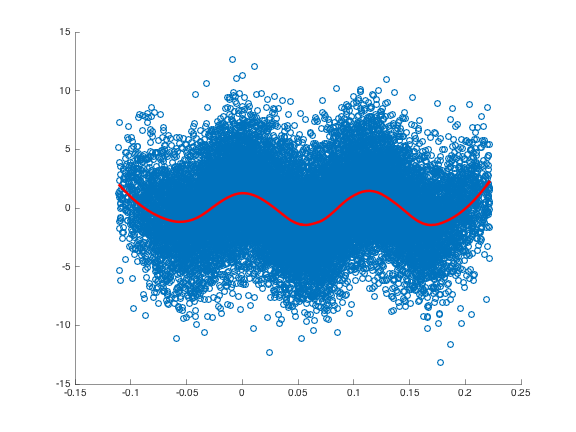
\includegraphics[width=.5\linewidth]{shape}
  \caption{Probable shape from one of the beating movies. }
  \label{fig:shape}
\end{figure}

\subsection{Extracting Probable Beating Pattern}

To estimate the probable shape of the beating pattern we make use of the results from the frequency analysis using the FFT. We select the ROIs with the most common dominant frequencies and high activity to regress the beating shape. Before using locally weighted linear least squares to estimate the shape we use the phase estimates to shift the samples in time such that they all have the same phase. The function implementing this procedure is \texttt{probableShapeFromData.m} and the corresponding header is shown in Listing \ref{shape}. An example result is shown in Figure \ref{fig:shape}.

\begin{minipage}{\linewidth}
  \begin{lstlisting}[caption={Function for extracting the probable beating pattern.}, label=shape]
function [ shape ] = probableShapeFromData( dominantFreqs, phase, data,...
    activity, fs )
%PROBABLESHAPEFROMDATA Computes the probable shape of the beating pattern 
%from the results of the FFT and the underlying data.
%Note: The FFT should be computed using ROI-size=1 for use with this 
%function.
% Input:
%   dominantFreqs - 2D array of size (w x h) with dominant frequencies per 
%                   pixel 
%   phase - 2D array of corresponding phases per pixel
%   data - 3D array of extracted video data of size (w x h x t)
%   activity - 2D array of activities phases per pixel
%   fs - Sampling frequency of the input data
% Output:
%   shape - Curve fitted to the data using smoothing-splines
% See also PERFORMFFT, COMPUTEENTROPY, ACTIVITYFROMPOWER.  
\end{lstlisting}
\end{minipage}


\subsection{Batch Processing of the Data}

The processing of the video data is possible in batches. Processing of videos takes place in two phases, first the data is extracted from videos contained in a folder with \texttt{batchExtractFolder.m} for further processing. Data is extracted for all videos contained in the specified folder including subfolders. In the second phase, the extracted data is then analysed with \texttt{batchAnalyseFolder.m}. This function coordinates the frequency and activity analysis and takes care of storing the results. Both functions can run parallel (if the required Toolbox is installed) leading to significant speed-ups on multiprocessor systems. The header of \texttt{batchExtractFolder.m} is shown in Listing \ref{extract} and the header of \texttt{batchAnalyseFolder.m} in Listing \ref{process}.


\begin{minipage}{\linewidth}
  \begin{lstlisting}[caption={Function for extracting data from videos.}, label=extract]
function batchExtractFolder( extractFolder, storeFolder, reload )
%BATCHEXTRACTFOLDER Extracts data of all the videos in the folder 
%extractFolder (including subfolders) and saves it to storeFolder for later 
%analysis. Note that if reload is set to false and the video has already 
%been extracted, the video will not be extracted again.
% Input:
%   folderPath - String indicating the path of the video-data
%   storeFolder - Folder where the extracted data should be stored
%   reload - Boolean value (already extracted videos skipped if false)
% See also EXTRACTVIDEODATA, SAVEEXTRACTEDDATA and ALREADYEXTRACTED.
\end{lstlisting}
\end{minipage}

\begin{minipage}{\linewidth}
  \begin{lstlisting}[caption={Function for analysing extracted data.}, label=process]
function batchAnalyseFolder( folderPath, fs, roiSize, resultsDir,...
    preProcess, method, waveletType )
%BATCHANALYSEFOLDER Anlayses all files in the given folder using the
%specified parameters and saves the results to the folder resultsDir.
% Input:
%   folderPath - Path to folder of exctracted video files to be analysed
%   fs - Sampling frequency of the data to be analysed
%   roiSize - Integer or vector [sx, sy] specifying the ROI-size
%   resultsDir - Path to directory where results should be stored
%   preProcess - Function handle for pre-processing function of extracted
%                data (e.g. denoising)
%   method - String indicating which method to use for analysis ("wt",
%            "fft" or "both")
%   waveletType - Specifies which wavelet to use for the wavelet transform.
%                 'morl' is used by default
% See also BATCHEXTRACTFOLDER, FILTER3D.
\end{lstlisting}
\end{minipage}


\subsection{GUI}

For a more flexible and convenient interpretation of the results we provide a GUI. Note that it is only used for the inspection of the results and not for running the analysis. Figure \ref{fig:gui} shows the layout of the GUI. Some of the special features of the GUI are the following:
\begin{itemize}
\item The available videos and ROIs for inspection are accessible via the two drop-down menus in the top-left.
\item The techniques used for the frequency and activity analysis can be switched via the buttons on the left.
\item Clicking on a ROI in the activity plot will show the corresponding frequency spectrum in the bottom centre plot.
\item In the dropdown-menus above the bottom-left and bottom-right figures you can choose which statistics or plots these figures should display.
\item The activity mask (top-right) can be manipulated via the two dropdown-menus above the figure. The mask influences some of the statistics, i.e. yellow ROI are included and blue ROI excluded.
\end{itemize}
 

\begin{figure}[h]
  \centering
  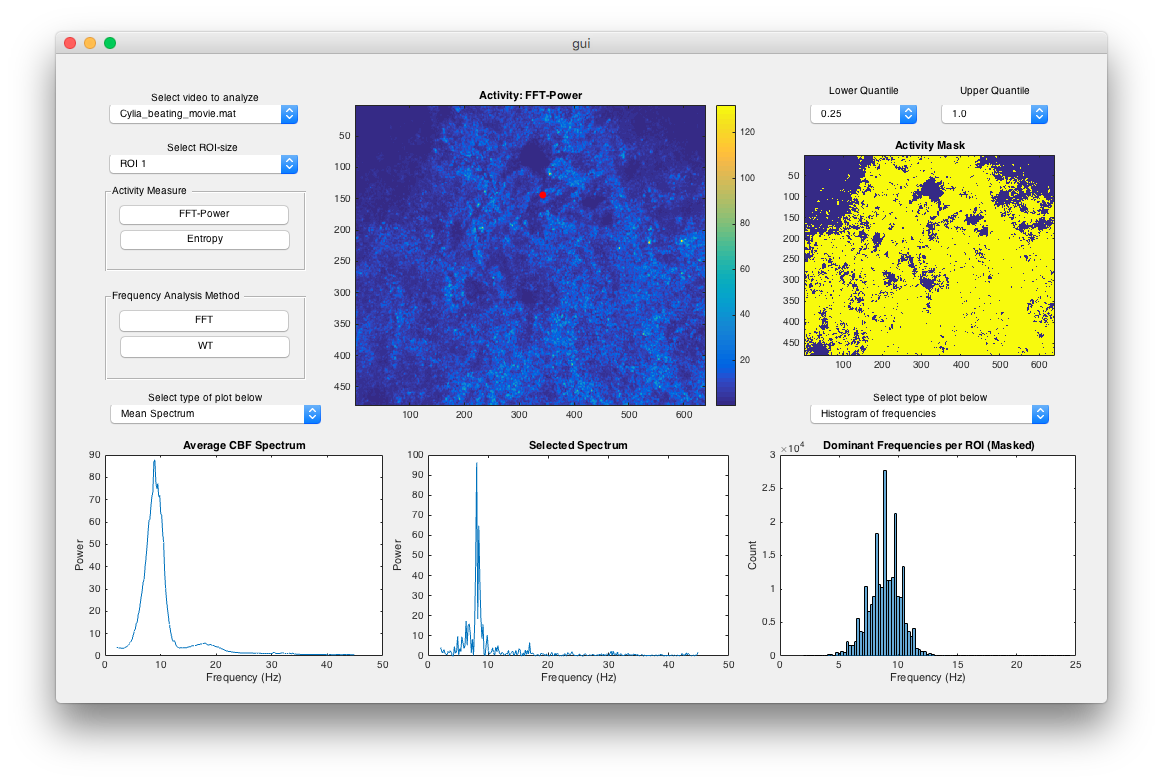
\includegraphics[width=0.9\linewidth]{GUI}
  \caption{The GUI which can be used to inspect the results of the analysis.}
  \label{fig:gui}
\end{figure}

%----------------------------------------------------------------------------------------
%	SECTION 4
%----------------------------------------------------------------------------------------

\section{Evaluation}

\subsection{Effect of ROI-Size on Performance}
\label{sec:effect-roi-size}

We compared the computation time required for the FFT and WT analysis for different ROI sizes on a single video. We tested with ROIs of size $1$, $[3, 4]$ and $[6, 8]$ on a 2.4 GHz Intel Core i5 MacBook Pro with 8 GB 1067 MHz DDR3 RAM. The results are plotted in Figure \ref{fig:computational-time}.

\pgfplotstableread{speed_results.dat}\speed
\begin{figure}[ht]
  \begin{minipage}{0.3\linewidth}
    \centering
    \pgfplotstableset{%
      fixed zerofill,
      precision=3,
      every head row/.style={before row=\toprule,after row=\midrule},
      every last row/.style={after row=\bottomrule}
    }
    \pgfplotstabletypeset[columns={FFT,WT}]\speed
    
  \end{minipage}
  \begin{minipage}{0.4\linewidth}
    \centering
    \begin{tikzpicture}[scale=1]
      \begin{axis}[
        scaled ticks=base 10:0,
        xlabel = {ROI sizes},
        ylabel = {Time (s)},
        title={Computational time of the FFT and WT},
        xtick = {1,2,3},
        xticklabels={{ROI $1$}, {ROI $[3, 4]$}, {ROI $[6, 8]$}},
        xticklabel style={rotate=45,anchor=east, scale=0.9}
        ]
        \addplot table[y = FFT] from \speed ; 
        \addlegendentry{FFT} ;
        \addplot table[y = WT] from \speed ;
        \addlegendentry{WT} ;    
      \end{axis}
    \end{tikzpicture}
  \end{minipage}
  \caption{Computational time of the FFT and WT for different ROI sizes}
  \label{fig:computational-time}
\end{figure}

We observe that computing the FFT pixel-wise takes approximately 2 minutes and 40 seconds, while it takes around 25 
minutes for the WT. However, as soon as we increase the ROI size, the computational time for the WT decreases
drastically. It should be noted that the computations were run with \texttt{batchAnalyseFolder}, hence the
times presented here are greater than if we had only used \texttt{performFFT} or \texttt{WTAnalysis}.

\begin{figure}[h]
  \centering
  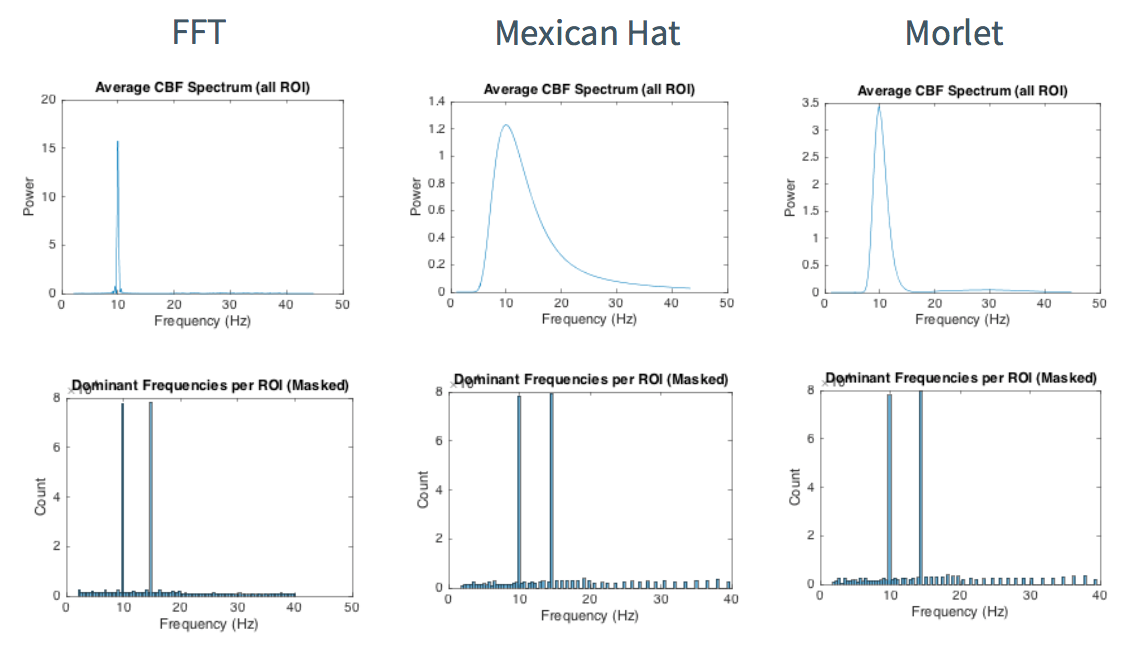
\includegraphics[width=0.8\linewidth]{compare}
  \caption{Comparison of results obtained with the FFT (left), WT with Mexican-Hat wavelet (middle) and WT with Morlet wavelet. }
  \label{fig:compare}
\end{figure}


\subsection{A Comparison of the Different Techniques}
\label{sec:comp-techn-used}

\paragraph{Frequency Analysis}

We compared results obtained with the FFT with results obtained with the WT on synthetic data to get an idea of the quality of the results. The synthetic example in this case is made up of high amplitude sinusoid at 10Hz and low amplitude sinusoids at 15Hz. Results are shown in Figure \ref{fig:compare}. We make the following observations:

\begin{enumerate}
\item The FFT is much more precise with respect to frequency analysis. We can clearly observe this in Figure \ref{fig:compare}. 
\item The results of the WT are highly dependent on the type of wavelet. The Morlet for example is much closer to the FFT than the Mexican-Hat wavelet.
\item FFT is much faster than WT especially at smaller ROI-sizes.
\item FFT provides us with phase information that we can use to compute the probable beating pattern.
\item WT allows time-frequency analysis.
\item WT is very customisable and so most likely the results with the WT can be improved through careful parameter tuning.
\end{enumerate}

From these observations we can conclude that if we are not interested in a time-frequency analysis of the signal we get no benefit from using the WT.

\paragraph{Activity analysis:}

We implemented two methods to analyse the activity of the video: using the FFT power and entropy. 
If the FFT was previously computed, then computing the activity with the FFT is
straightforward and very fast. The function computing the entropy has a $O(\mathtt{heigth} \times \mathtt{width}
\times \mathtt{time})$ complexity. The quality of the two techniques is quite different in that FFT power is much more sensible to the amplitude in the signal. 
If we're interested to only look at very strong beatings it is therefore more useful to look at the FFT-power. Conversely, if we are more interested in low amplitude signals the entropy seems like the better choice. 


%----------------------------------------------------------------------------------------
%	SECTION 6
%----------------------------------------------------------------------------------------

\section{Recommendations}

\subsection{Statement of Recommendations}
As stated in Subsection \ref{sec:comp-techn-used} we recommend the use of the FFT for the frequency analysis due to its much better frequency resolution and lower computation time. If time-frequency analysis becomes of interest the WT will likely be the better option.   

We also recommend a more rigorous testing and comparison of the methods based on clearly defined features in the results and in collaboration with the client.

\subsection{Limitations}
In our opinion, the main limitation of our work is that the tool was not yet tested in the wild, i.e. in a real experiment with the intended users. This will mostly likely uncover several possibilities for further optimisation, be it concerning usability, implementation of additional features or improvements of existing functionality. 

\subsection{Outstanding Issues and Perspective for Future Work}
One idea for future improvement of the tool would be to allow the user to specify the mask in the GUI by hand, i.e. through mouse-clicks on the activity plot of the GUI for example. 
We could also imagine that other metrics besides the activity might be interesting in specifying the mask.

Concerning the estimation of the beating pattern, we believe that it could most likely be improved through more careful selection of the data used for the fitting. Concretely it might be beneficial to detect and exclude outliers and only consider samples that have roughly the same amplitude.


%----------------------------------------------------------------------------------------


\end{document}